\documentclass[12pt,a4paper,openright]{article}
\usepackage[utf8]{inputenc}
\usepackage[spanish]{babel}
\usepackage{amsmath}
\usepackage{amsfonts}
\usepackage{amssymb}
\usepackage{graphicx}
\usepackage[left=2cm,right=2cm,top=2cm,bottom=2cm]{geometry}

\title{Reporte De Actividad 3}
\author{Francisco Javier Real Santoscoy\\
Departamento de Física\\
Universidad de Sonora}
\date {01 de Diciembre del 2015}
\begin{document}
\maketitle
\section{Introducción}
Fortran es un lenguaje de programación de alto nivel de propósito general, procedimental e imperativo, que está especialmente adaptado al cálculo numérico y a la computación científica. Desarrollado originalmente por IBM en 1957 para el equipo IBM 704, y usado para aplicaciones científicas y de ingeniería, el FORTRAN vino a dominar esta área de la programación desde el principio y ha estado en uso continuo por más de medio siglo en áreas de cómputo intensivo tales como la predicción numérica del tiempo, análisis de elementos finitos, dinámica de fluidos computacional (CFD), física computacional y química computacional. Es uno de los lenguajes más populares en el área de la computación de alto rendimiento y es el lenguaje usado para programas que evalúan el desempeño (benchmark) y el ranking de los supercomputadores más rápidos del mundo.
El FORTRAN (una palabra derivada de The IBM Mathematical Formula Translating System) abarca un linaje de versiones, cada una de las cuales evolucionó para añadir extensiones al lenguaje mientras que usualmente retenía compatibilidad con las versiones previas. Versiones sucesivas han añadido soporte para procesamiento de datos basados en caracteres (FORTRAN 77), programación de arreglos, programación modular y programación orientada a objetos (Fortran 90/95), y programación genérica (Fortran 2003).
\section{Actividad a Realizar}
En esta actividad trataremos de elaborar nuestro primer programa en Fortran para estudiar una función, que posee todas sus derivadas de orden superior.
Tomaremos un caso sencillo de la función f(x) = sin(x). Se te proporciona el programa inicial sinfunct.f90:

\begin{verbatim}
! Este programa calcula la función Sin(x) en el intervalo [0, 2 pi]
! Definimos el nombre del programa Fortran. Le damos el mismo nombre que el 
! programa fuente sinfunct.f90 
program sinfunct
! Tres espacios de sangría
! No suponemos nada
  implicit none 
! Definimos todas la variables que vamos a utilizar y su tipo
  integer :: i, npts ! npts es el número de puntos en el intervalo [0,2pi]
  real :: x, f_x,dx  ! La variable, una función f(x) y el incremento dx
  real, parameter :: pi = 4.0 * atan (1.0) ! Dejamos que la máquina calcule pi 
  print *,  'Dame el número de puntos en el intervalo npts= '
  read(*,*) npts 
  dx = (2.0 * pi) /float(npts) ! dx es el incremento en el eje x
  write(*,*) 'dx= ', dx 
  x = 0.0 ! Es el límite inferior del intervalo de interés
  ! Comenzaremos evaluando f(x) desde x=0, y debemos incluir también x=2*pi
! Inciamos un "loop", notemos la sangría dentro del loop. !
  do i = 1, npts+1, 1 
     x = dx * float(i-1)
     f_x = sin(x)
     write(*,*) i, x , f_x
enddo
! termina el loop 
end program sinfunct 
! termina el programa
\end{verbatim}
\section{Resultados}
Despues de realizar lo indicado en la actividad logramos identificar donde la fincion de sen(x) se hace 0. Como tambien aproximamos a la funcion utilizando la Serie de Taylor. A continuación se pueden ver la grafica del seno y coseno ya aproximada de 0 a 2pi.






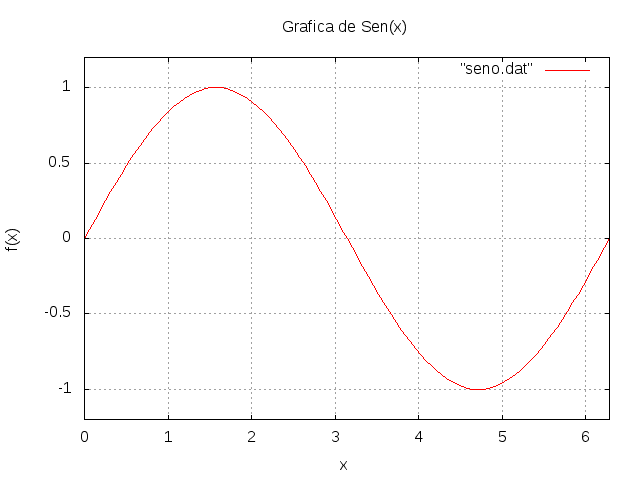
\includegraphics[scale=1]{sen.png} 
\begin{figure}[htb]
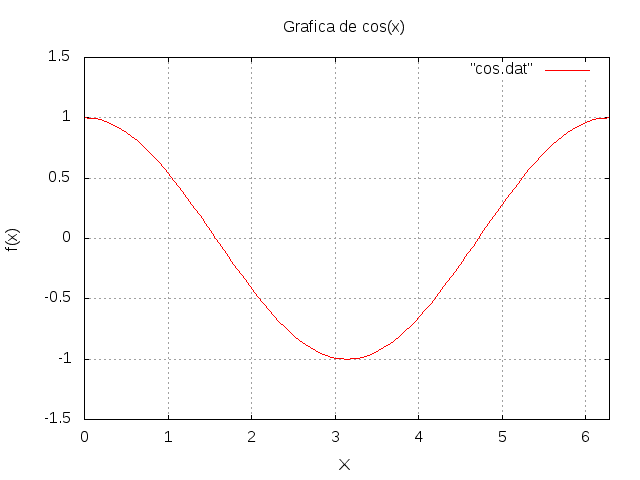
\includegraphics[scale=1]{coseno.png} 
\caption{Gráfica del Seno}
\end{figure}
\end{document}